% !TeX spellcheck = en_US
% !TEX root = ../thesis-example.tex
%
\section{Camera Input Lag}

After the rather simple integration of the keyed video signal into the scene, 
where the 3D environment is used as background, an offset between the render 
image from the scene and captured footage from the camera can be observed due 
to the pipeline from the capturing device through video converting of the 
Inogeni 4KUSB3 bound to the systems webcam API.

\begin{figure}[htb]
	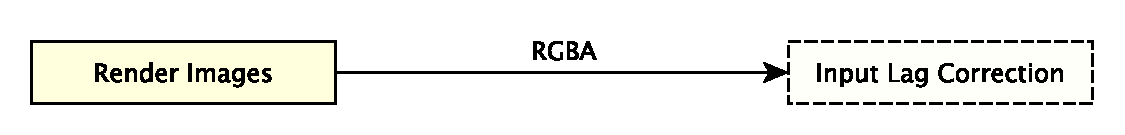
\includegraphics[width=\textwidth]{_raw_resources/pipeline_steps/4_2_swapper.pdf}
	\caption{The initial step upon receiving the camera image is to adjust the 
	time drift between engine renderings and video capture}
	\label{fig:steps:swapper}
\end{figure}

After consulting the specification of the Inogeni 4K2USB3 it states that a 
conversion from any HDMI video source takes two intrinsic frames for encoding. 
The camera framerate is $F_C = 25 \frac{frames}{second}$. This would mean, in 
theory:

\eq{offsets:timing:1}{
	t = \frac{2}{F_C}
}

Assuming 25 frames per second, that is $\frac{1}{30}s$:

\eq{offsets:timing:2}{
	t =  \frac{2}{25 \frac{frame}{second}}
}

\eq{offsets:timing:3}{
	t = 80ms
}

The observed offset from camera to engine is far longer in reality and remains 
at about 260ms after testing this setup and observing the drift, therefore 
seeing noticeable in any motion video as shown in figure 
\ref{fig:offsets:example}.

\begin{figure}[htbp]
	\caption[Aligned and unaligned frames]{Visual comparison between unaligned 
	and aligned frames\footnotemark}
	\label{fig:offsets:example}
	\begin{subfigure}[t]{.45\textwidth}
		\centering
		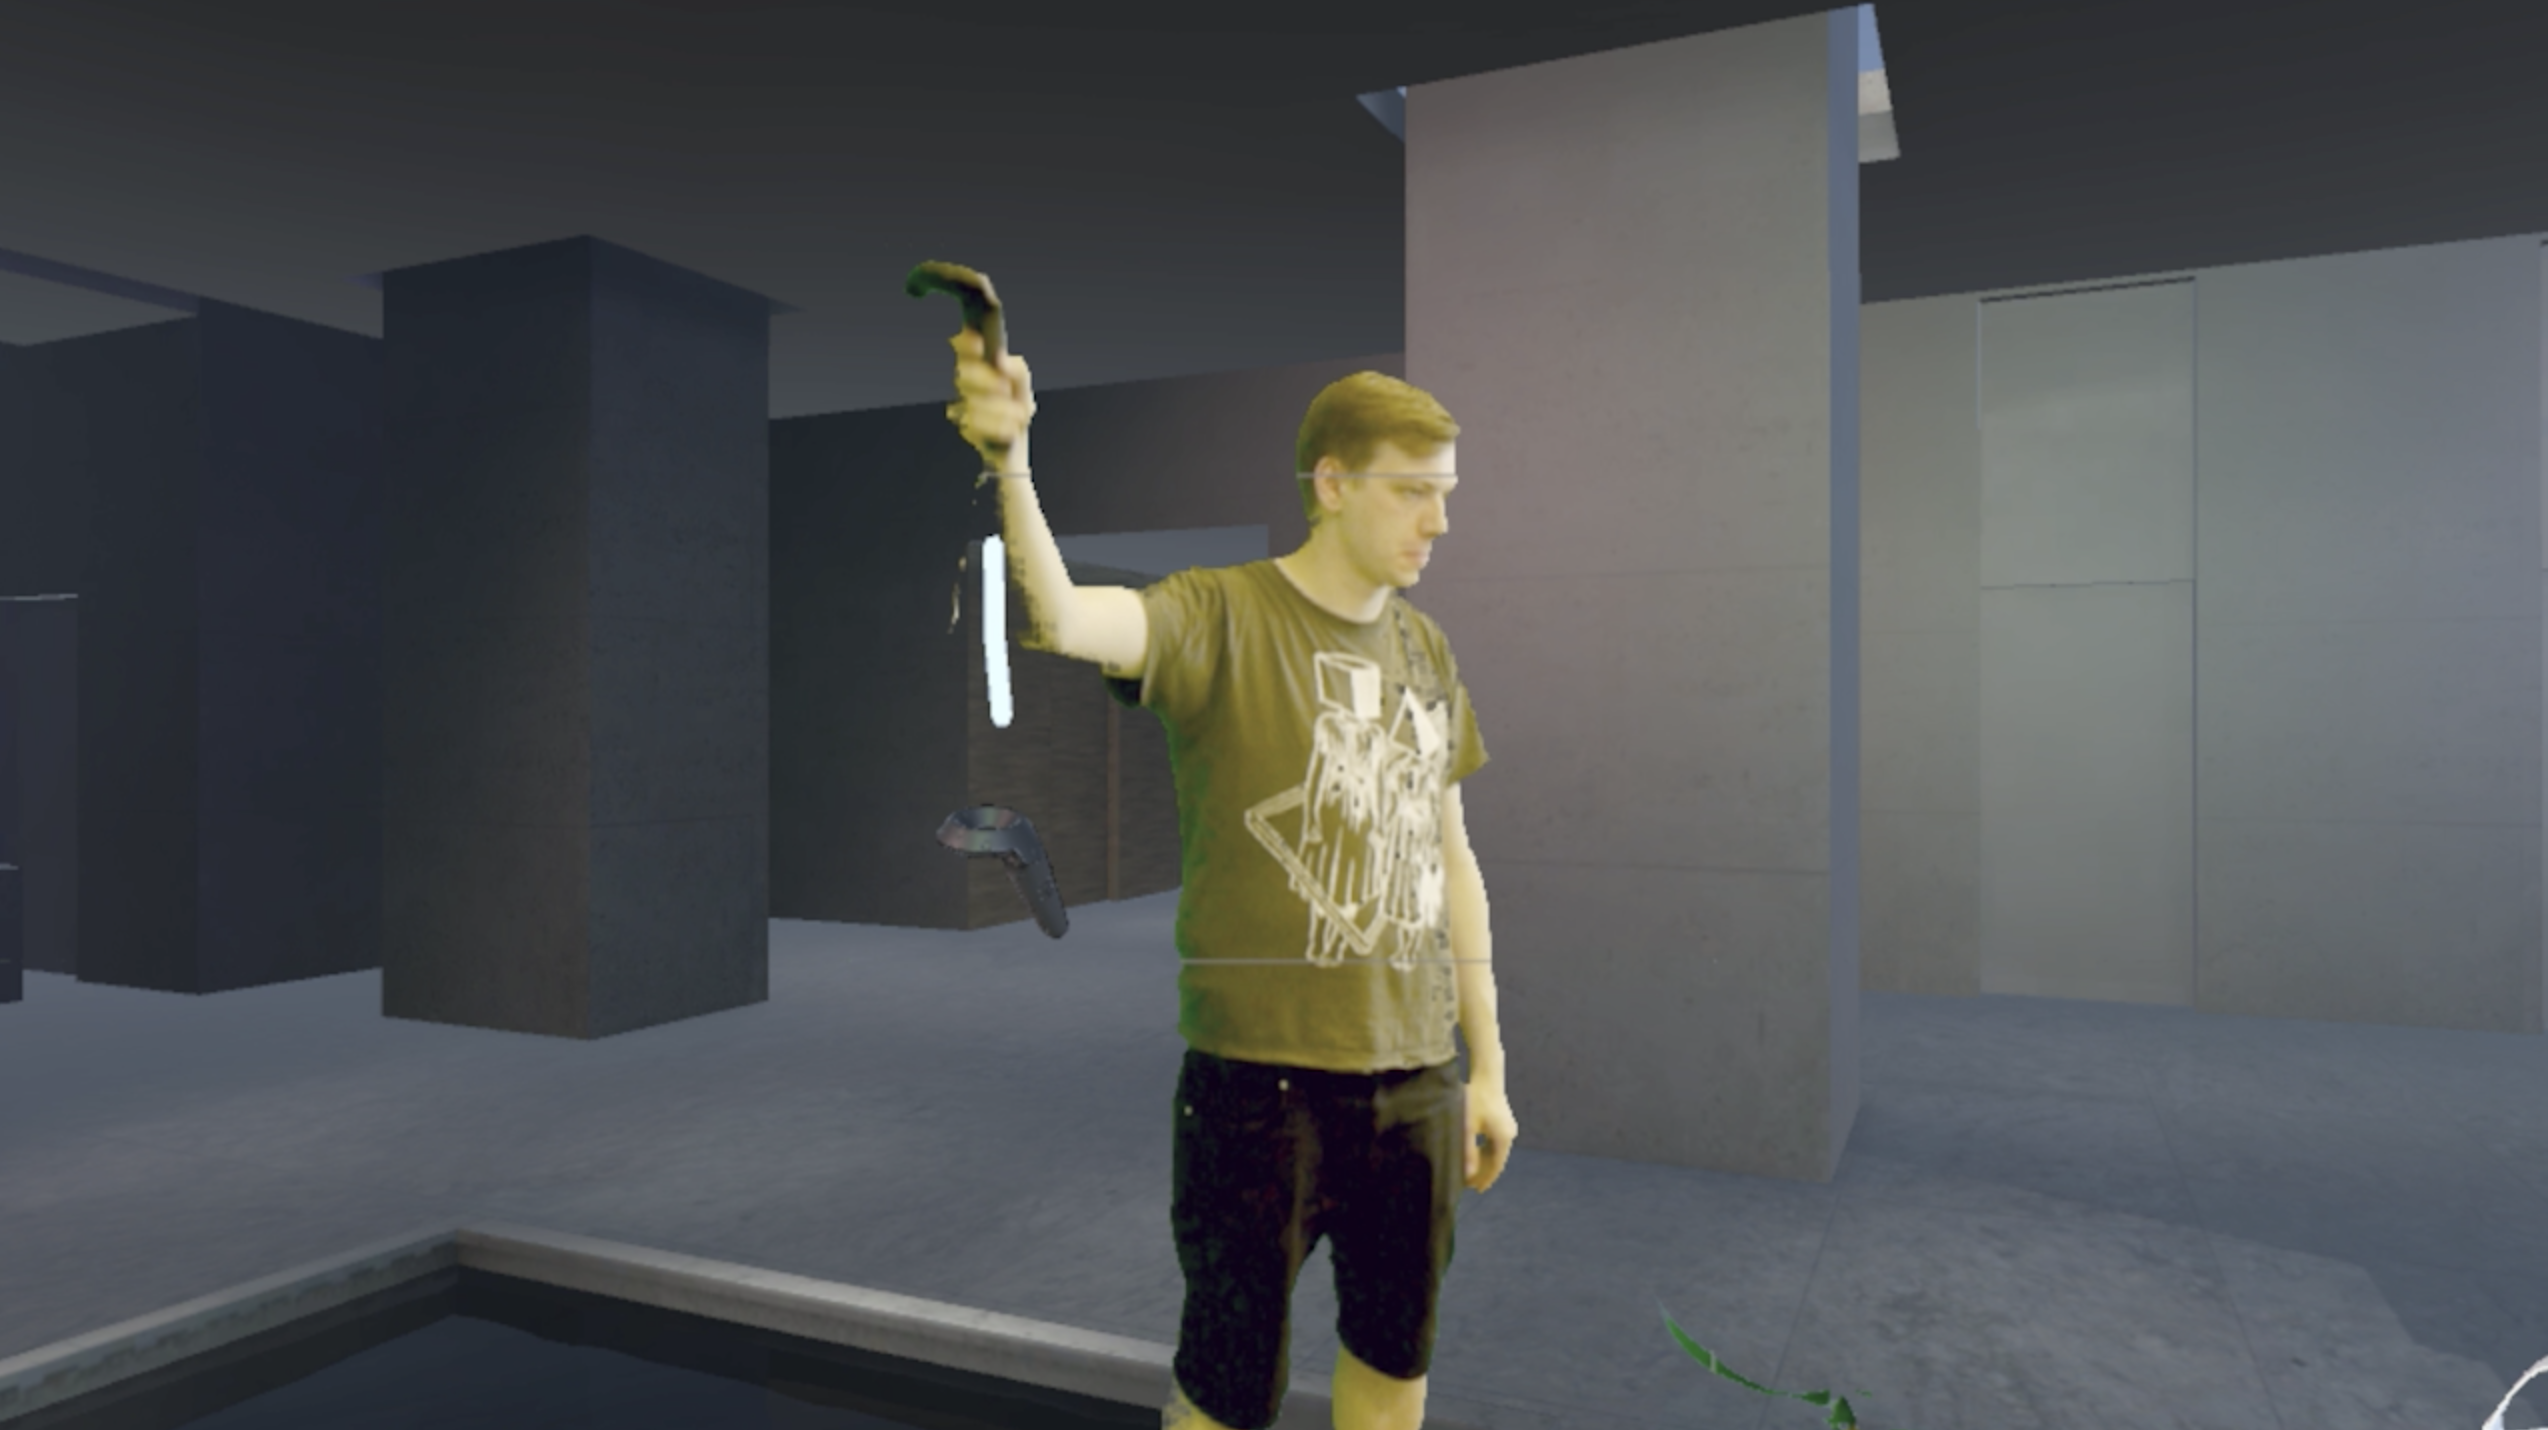
\includegraphics[width=\textwidth]{gfx/offsets/not_aligned.png}
		\caption{Before video and engine frames have been aligned, there is a 
		noticable difference in motion}
	\end{subfigure}
	\begin{subfigure}[t]{.45\textwidth}
		\centering
		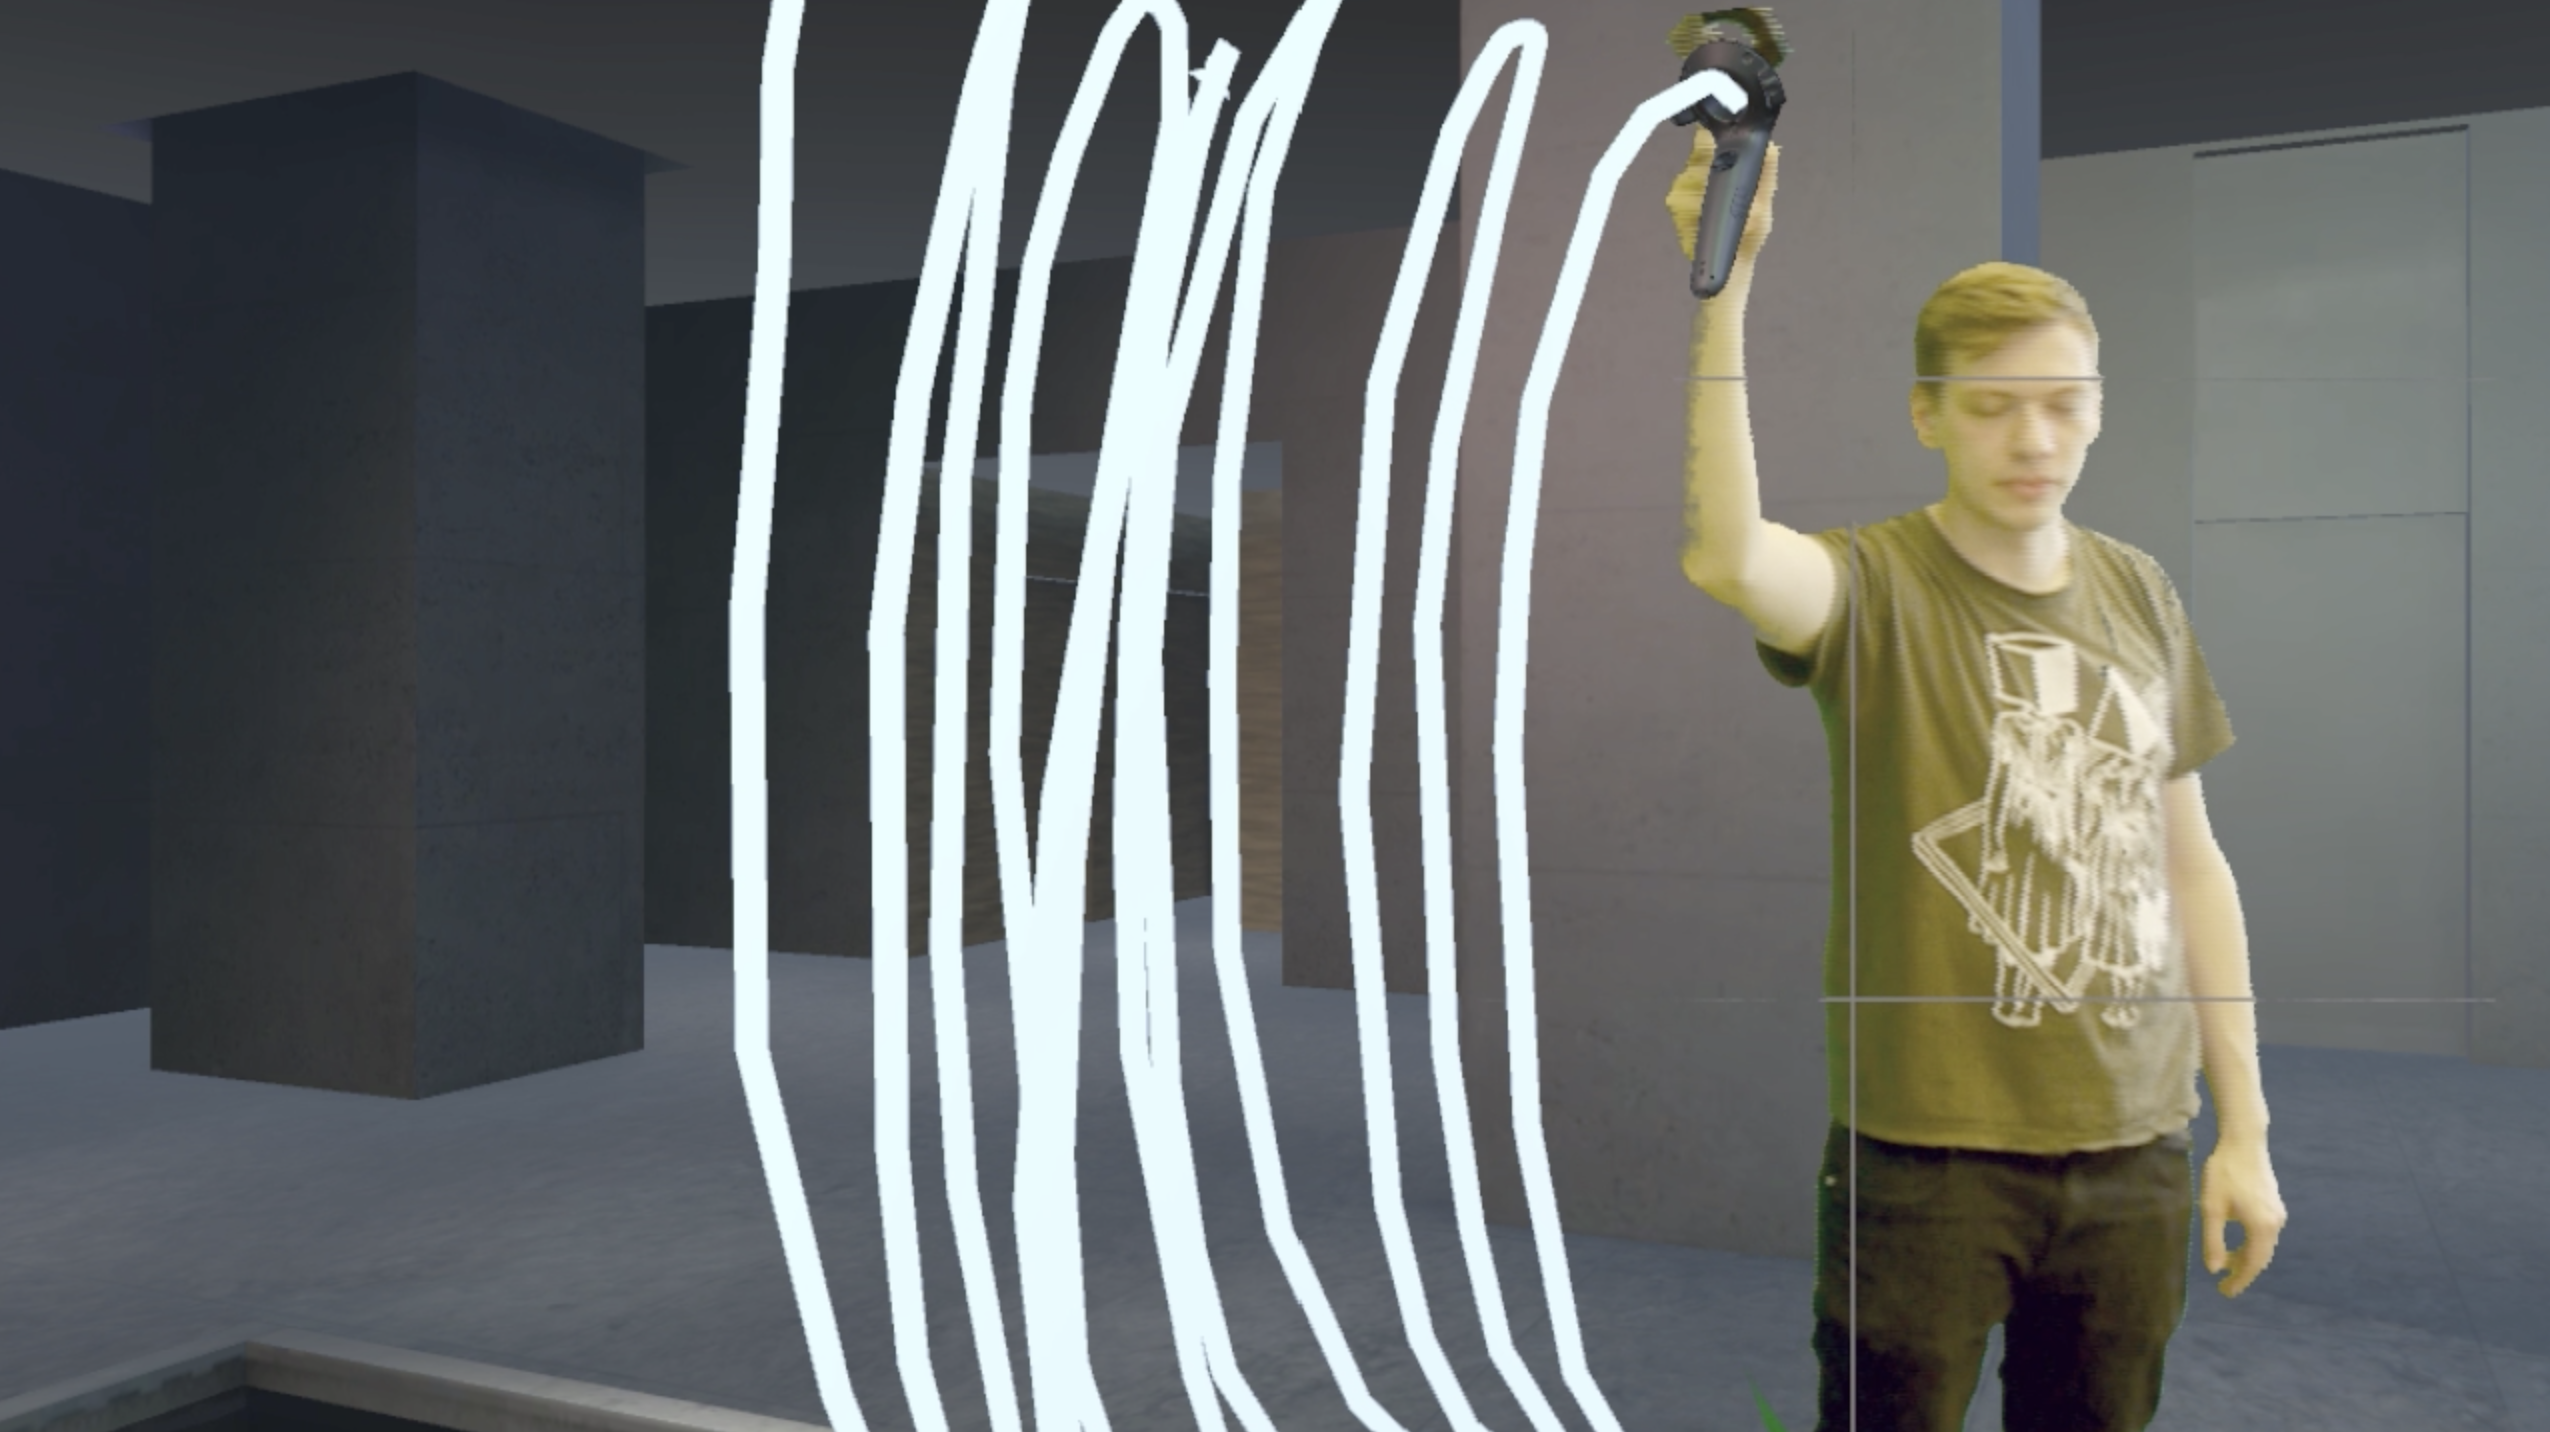
\includegraphics[width=\textwidth]{gfx/offsets/aligned.png}
		\caption{After aligning frames the motion in engine and video capture 
		are in sync}
	\end{subfigure}
\end{figure}

\footnotetext{a video example is provided on the additional storage device}

To mitigate this offset there are two options:

\begin{my_list}
	\item Change the camera setup - for example a direct webcam, which 
	usually has a lower input latency, ranging between 5 - 250ms. That would 
	degrade the image quality significantly but would enable better rendering 
	conditions inside the engine.
	\item Capture virtual images of the 3D environment and keep them on the GPU 
	until a real world video frame is loaded onto the GPU for usage - assuming 
	that the time drift is constant. This keeps the image quality but needs 
	significant effort to reproduce the rendering conditions at the engine time 
	when a video frame was taken.
\end{my_list}

The proposed solution for this thesis uses the secondary option, since it is 
able to minimize any kind of constant offset between render image and a video 
stream, the hardware setup can stay dynamic\footnote{as long as it is provided 
by the systems webcam API} and it is little to no difference by switching to a 
webcam-integrated solution than an encoding box and the resulting displayed 
image has imperceptible differences to the former variant. It is therefore more 
user friendly and can accommodate for a wide range of video devices.

\begin{figure}[htb]
	\centering
	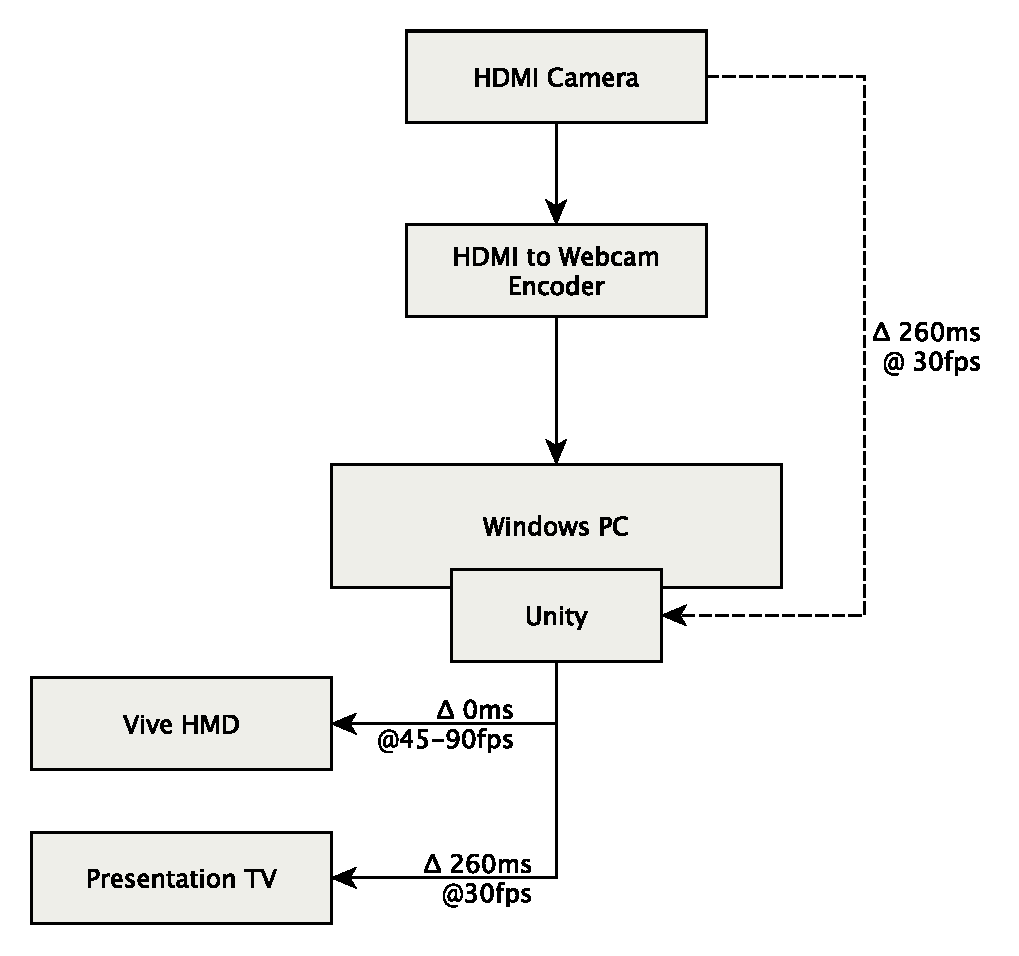
\includegraphics[width=.85\textwidth]{gfx/FPS-Timing-Components.pdf}
	\caption{Components in considering video input lag and frame rates. While 
	latencies between each components cannot measured, it is observed with help 
	of an interactive VR object.}
	\label{fig:offsets:components}
\end{figure}

Based on the component diagram \ref{fig:offsets:components} there are two 
important takeaways: 

\begin{my_list}
	\item There is an input latency between the production camera and the Unity 
	Engine, which in turn needs to be reproduced on the mixed reality 
	presenting device
	\item Frame rates between the Vive HMD and the presentation TV differ 
	because the TV's frame rate should be matched to the input video feed from 
	the camera (see section \ref{sec:framejitter})
\end{my_list}

At the time of writing Unity does not support dynamic frame rates on multiple 
viewports\footnote{A viewport can be either a D3D, OpenGL or Metal 3D context}.
\newline
It is possible to manually initiate a virtual camera's rendering, however, this 
causes the render loop to mistime and yields inconsistent frame timings inside 
the HMD and is no different between the average GPU load to display the 
presentation TV's viewport. It makes no perceptive difference if a scene 
renders 11ms twice and then falls down to 22ms once --- however the observed 
stuttering is a major degradation of the actors experience and often times 
causes motion sickness (fig. \ref{fig:cameralag:mistiming}).

\begin{figure}[htbp]
	\caption{Differences in performance based on rendering strategy}
	\label{fig:cameralag:mistiming}
	\begin{subfigure}[t]{\textwidth}
		\centering
		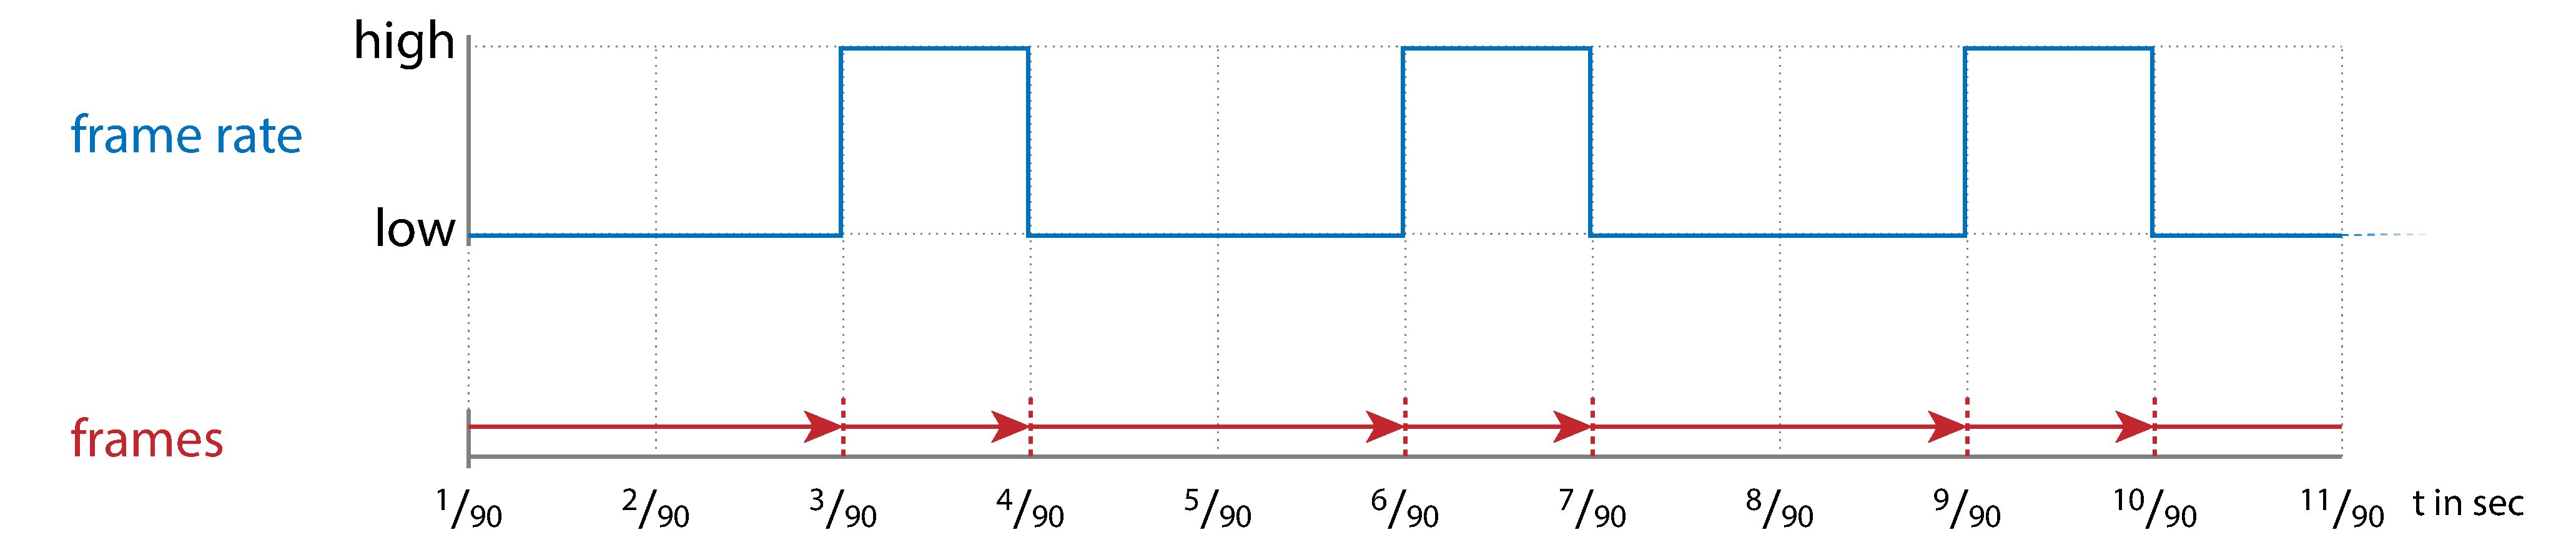
\includegraphics[width=\textwidth]{gfx/mistiming/variable.pdf}
		\caption{Initiating rendering when needed can cause stuttering 
		performance inside the headset, yielding motion sickness for the VR 
		actor}
	\end{subfigure}
	\begin{subfigure}[t]{\textwidth}
		\centering
		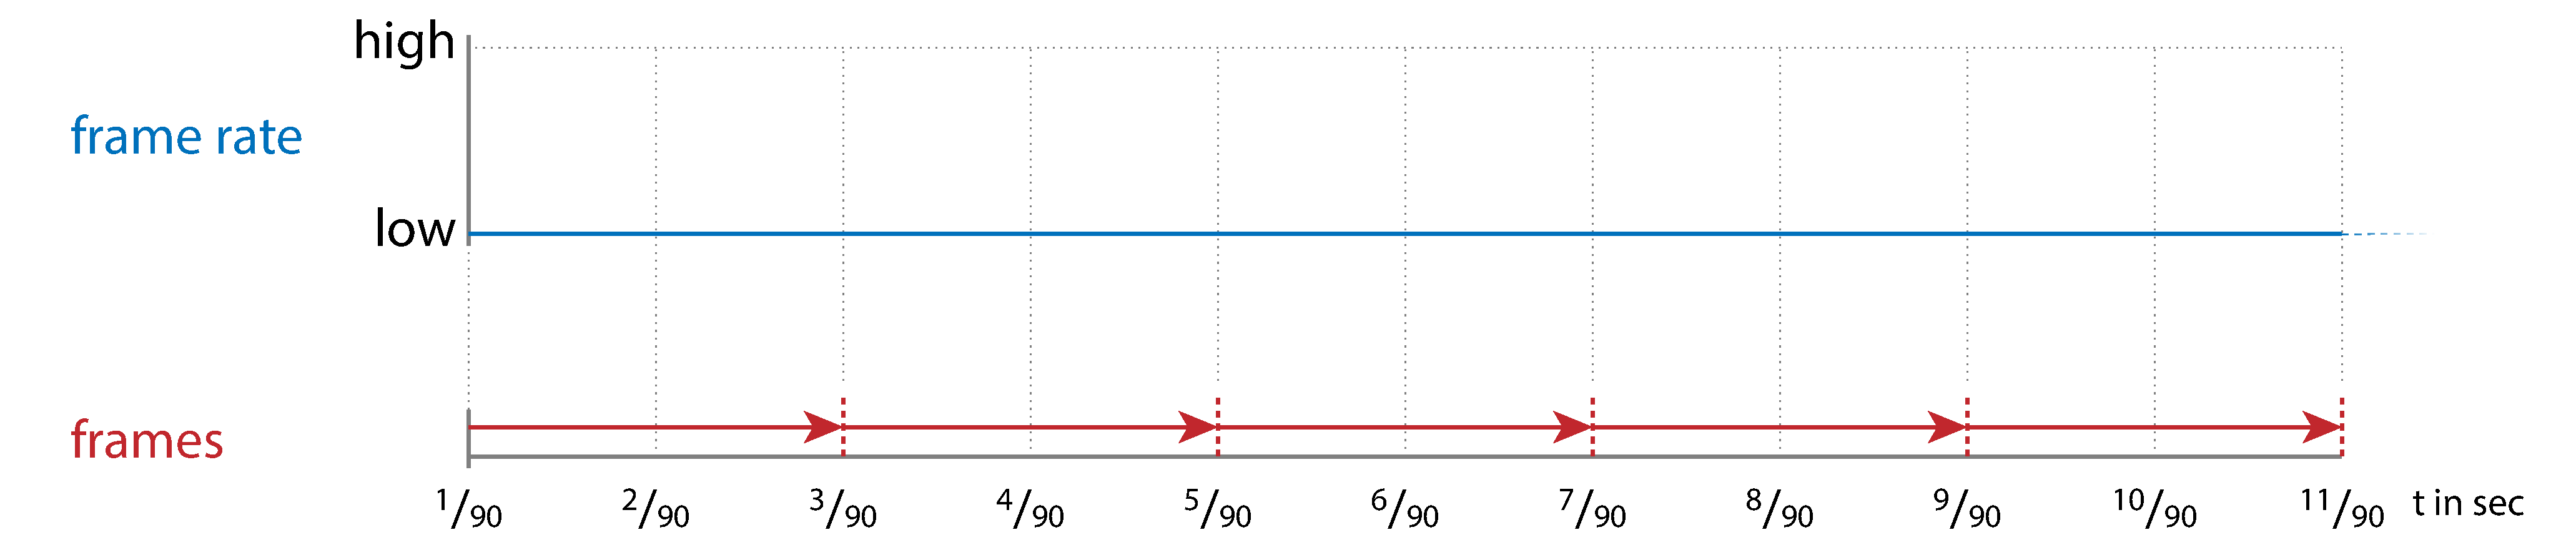
\includegraphics[width=\textwidth]{gfx/mistiming/stable.pdf}
		\caption{Consistent poor performance is less irritating for the VR 
		actor and makes no difference for a Mixed Reality composition}
	\end{subfigure}
\end{figure}

To conclude: The software has to store a set amount of \gls{framebuffer}s and 
cycle them at the right frame to guarantee minimal delays between camera and 3D 
environment, thus realigning the observed time drift between the engine and 
captured video frames.

Noteworthy is that the render loop can be 45 or 90 fps, depending on scene 
complexity, overall system performance or - especially in case of Unitys 
outdated C\# version - garbage collection, that could halt the engine for a 
significant amount of time. To account for this, a strategy is needed in which 
Unity's \code{Time.deltaTime} property is used, which describes the time 
between last and current frame, allowing for accurate timing how framebuffers 
have to be handled and swapped.

\subsection{Framebuffer Swapper Implementation}

Unity has a well engineered engine loop, where it can perform different 
operations at specific steps of the main engine execution\footnote{For more 
detail about Unity's core loop there is a flowchart in the Appendix 
\ref{app:engineloop}, depicting MonoBehaviors life cycle.}. As 
initial data needed is \code{cameraFPS}, \code{cameraOffset} and 
\code{Time.deltaTime}. With that input it is possible to calculate the 
\code{frameWindow}, which is the time of one displayed frame and 
\code{delay}, which is the time drift in frames between camera and engine:

\eq{eq:swapper:vars:1}{
	\textnormal{frameWindow} = \frac{1}{\textnormal{cameraFPS}}
}

\eq{eq:swapper:vars:2}{
	\textnormal{delay} =
		\frac{\textnormal{cameraOffset}}{\textnormal{frameWindow}}
}

\subsection{Double Access Ringbuffer}

In Unity's case a framebuffer is called \code{\gls{render texture}}. To spare 
memory and bandwidth overhead it is possible to reuse previously allocated 
\code{RenderTextures} by overwriting the second oldest \code{RenderTexture} and 
compositing a mixed reality image with the oldest \code{RenderTexture}(see  
Figure \ref{fig:offsets:framesquashing}).

\begin{figure}[ht]
	\centering
	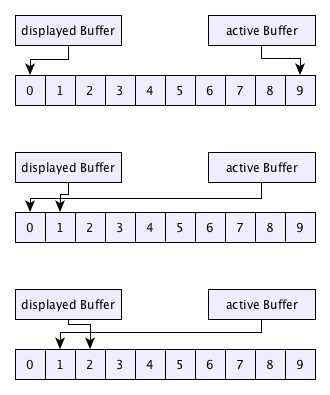
\includegraphics[width=.5\textwidth]{gfx/ringbuffer_schematics.png}
	\caption{Schema of an the ringbuffer}
	\label{fig:offsets:ringbuffer}
\end{figure}

To accommodate for that behavior we have to write frame data into the current 
index and display the frame on its next index. After that step is taken we 
increment by one. This way we’re overwriting the oldest seen 
\code{RenderTexture} and show the one written to the next index. A reference 
implementation can be found in appendix \ref{app:darbi}.